%%%%% Magnetisches Feld %%%%%
%%  %%


%Some sample text to be displayed above the first subsection

%\subsection{Prinzip}

%Ein Zyklotron besteht aus Zwei hohlen, halbzylindrischen und Duanden an denen eine Spannung mit unterschiedlichem Vorzeichen anliegt, und darüber bzw. darunter liegende Magneten, die ein homogenes Magnetfeld erzeugen. Zudem gibt es einen Einlass und einen Auslass für Teilchen.

%\begin{wrapfigure}{r}{0.4\textwidth} \label{Zyklo}
%
%	\vspace{-10pt}
%	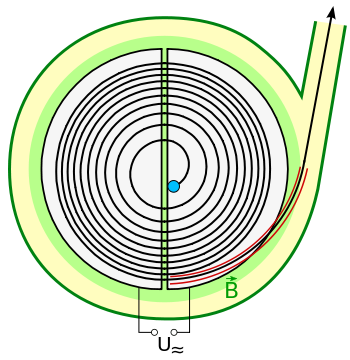
\includegraphics[width=0.35\textwidth]{Zyklotron_Prinzipskizze02.png}
%	\vspace{-13pt}
%	\caption{Prinzipskizze eines Zyklotrons}
%	\vspace{-5pt}	
%	
%\end{wrapfigure}

%\subsubsection{Anwendung}

% Some Formula:

%\begin{equation}
%	x= \frac{y \cdot 13 \pi z}
%			{\cos \alpha}
%\end{equation}

%%%%%%%%%%%%%%%%%%%%%%%
% Eigentlicher Beginn %
%%%%%%%%%%%%%%%%%%%%%%%

\subsection{Faustregel}	\label{subsec:Faustregel}

Als Eselsbrücke zur Bestimmung der Richtung der Feldlinien um den stromdurchflossenen Leiter kann die \glqq Faustregel\grqq{} herangezogen werden. Diese besagt, dass bei der physikalischen Stromrichtung (auch Elektronenflussrichtung genannt) die Feldlinien in Richtung der Fingerspitzen der linken Hand verlaufen, wenn der nur der Daumen abgespreizt wird und die Flussrichtung angibt.

Für die technische Stromrichtung gilt dieselbe Regel, bloß, dass mit der rechten Faust verfahren wird.

\begin{leftbar}
	Wichtig! Die physikalische Stromrichtung geht von der Bewegung der Elektronen, also der negativen Ladung aus. Diese fließen vom Minuspol zum Pluspol. Die technische Stromrichtung dagegen geht davon aus, dass die positiven Ladungen sich vom Pluspol zum Minuspol bewegen. Durch die Verwendung gespiegelter Handregeln (die jeweils andere Hand wird genommen) bleiben die Effekte jedoch dieselben. 
	
	Allgemein wird in der Physik die physikalische Stromrichtung und damit die \emph{linken} Handregeln bevorzugt, da es auch wirklich die Elektronen sind, die sich in einem Leiter bewegen.
\end{leftbar}

\subsection{Dauermagneten}  	\label{subsec:DauermagnetFeld}

 \hfill

\begin{figure}[ht!]
	\centering
	\begin{minipage}[b]{0.4\linewidth}
    	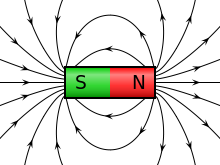
\includegraphics[width=\textwidth]{Stabmagnet}
		\caption{Das Magnetfeld um einen Stabmagnet.}
	\end{minipage}
	\quad
	\begin{minipage}[b]{0.4\linewidth}
    	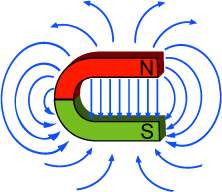
\includegraphics[width=0.6\textwidth]{Hufeisen}
		\caption{Das Magnetfeld an einem Hufeinenmagnet. Interessant ist der homogene Bereich zwischen den Schenkeln.}
	\end{minipage}
\end{figure}


\subsection{Gerader Leiter} 
\footnote{\url{https://lp.uni-goettingen.de/get/text/3791}} 
\footnote{„Gerader leiter“ von Talos aus der deutschsprachigen Wikipedia. Lizenziert unter CC BY-SA 3.0 über Wikimedia Commons - \url{https://commons.wikimedia.org/wiki/File:Gerader_leiter.svg}} 
\footnote{„Stromschleife“ von 30px MovGP0 - selbst erstellt mit Inkscape. Lizenziert unter CC BY-SA 2.0 de über Wikimedia Commons - \url{https://commons.wikimedia.org/wiki/File:Stromschleife.svg}} 
\label{subsec:GeraderLeiterFeld}

\hfill

\begin{figure}[ht!]
	\centering
	\begin{minipage}[b]{0.4\linewidth}
   	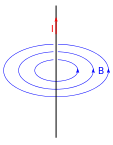
\includegraphics[width=\textwidth]{GeraderLeiter}
		\caption{Das Magnetfeld um einen geraden Leitern. $I$ zeigt die \emph{technische} Stromrichtung an.}
	\end{minipage}
	\quad
	\begin{minipage}[b]{0.4\linewidth}
    	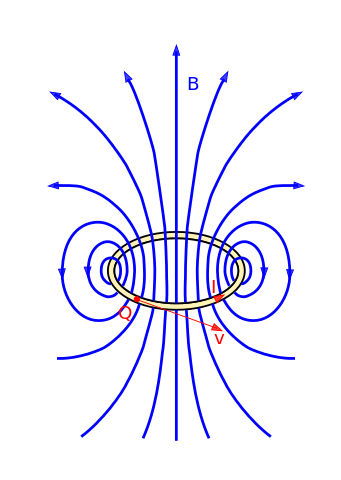
\includegraphics[width=\textwidth]{Stromschleife}
	\caption{Das Magnetfeld um eine Leiterschleife (Spule mit nur einer Windung). Man nehme Notiz von der Art, wie sich die einzelnen Feldlinien um den Leiter herum in der Mitte zu einem Bündel Feldlinien akkumulieren. $Q$ zeigt die \emph{technische} Stromrichtung an.}
	\end{minipage}
\end{figure}

\newpage

\subsection{Spule} \label{subsec:MFeldSpule}
\footnote{„VFPt cylindrical coil real“ von Geek3 - Eigenes WerkThis plot was created with VectorFieldPlot. Lizenziert unter CC BY-SA 3.0 über Wikimedia Commons - \url{https://commons.wikimedia.org/wiki/File:VFPt_cylindrical_coil_real.svg}}
\label{subsec:Spule}

\hfill

\begin{figure}[ht!]
	\centering
   	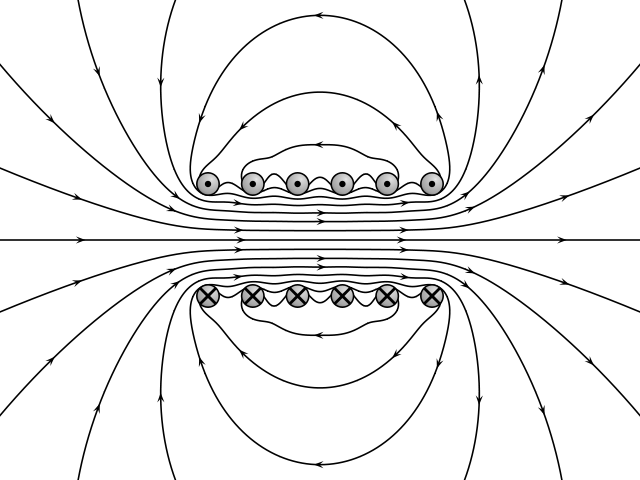
\includegraphics[width=0.8\textwidth]{Spule}
		\caption{Das Magnetfeld im Inneren einer Spule. Im Querschnitt zeigt $\otimes$ den technischen Stromfluss in die Ebene an. Vergleichbar mit der Leiterschleife, aber mit deutlich homogenerem Fluss im Inneren.}
\end{figure}



